\chapter{INTRODUCTION} \label{chap:intro}
 
 This document provides a simple template of how the provided
 \verb+iitmdiss.cls+ \LaTeX\ class is to be used.  Also provided are
 several useful tips to do various things that might be of use when you
 write your thesis.
 
 Before reading any further please note that you are strongly advised
 against changing any of the formatting options used in the class
 provided in this directory, unless you are absolutely sure that it
 does not violate the IITM formatting guidelines.  \emph{Please do not
   change the margins or the spacing.}  If you do change the formatting
 you are on your own (don't blame me if you need to reprint your entire
 thesis).  In the case that you do change the formatting despite these
 warnings, the least I ask is that you do not redistribute your style
 files to your friends (or enemies).
 
 It is also a good idea to take a quick look at the formatting
 guidelines.  Your office or advisor should have a copy.  If they
 don't, pester them, they really should have the formatting guidelines
 readily available somewhere.
 
 To compile your sources run the following from the command line:
 \begin{verbatim}
 % latex thesis.tex
 % bibtex thesis
 % latex thesis.tex
 % latex thesis.tex
 \end{verbatim}
 Modify this suitably for your sources.
 
 To generate PDF's with the links from the \verb+hyperref+ package use
 the following command:
 \begin{verbatim}
 % pdflatex thesis.tex
 \end{verbatim}
 
 \section{Package Options}
 
 Use this thesis as a basic template to format your thesis.  The
 \verb+iitmdiss+ class can be used by simply using something like this:
 \begin{verbatim}
 \documentclass[PhD]{iitmdiss}  
 \end{verbatim}
 
 To change the title page for different degrees just change the option
 from \verb+PhD+ to one of \verb+MS+, \verb+MTech+ or \verb+BTech+.
 The dual degree pages are not supported yet but should be quite easy
 to add.  The title page formatting really depends on how large or
 small your thesis title is.  Consequently it might require some hand
 tuning.  Edit your version of \verb+iitmdiss.cls+ suitably to do this.
 I recommend that this be done once your title is final.
 
 To write a synopsis simply use the \verb+synopsis.tex+ file as a
 simple template.  The synopsis option turns this on and can be used as
 shown below.
 \begin{verbatim}
 \documentclass[PhD,synopsis]{iitmdiss}                                
 \end{verbatim}
 
 Once again the title page may require some small amount of fine
 tuning.  This is again easily done by editing the class file.
 
 This sample file uses the \verb+hyperref+ package that makes all
 labels and references clickable in both the generated DVI and PDF
 files.  These are very useful when reading the document online and do
 not affect the output when the files are printed.
 
 
 \section{Example Figures and tables}
 
 \Cref{fig:point_mut} shows a simple figure for illustration along with
 a long caption.  The formatting of the caption text is automatically
 single spaced and indented. \Cref{tab:sample} shows a sample
 table with the caption placed correctly.  The caption for this should
 always be placed before the table as shown in the example.

\begin{figure}[htp]
  \centering
  \begin{subfigure}{\textwidth}
    \centering
    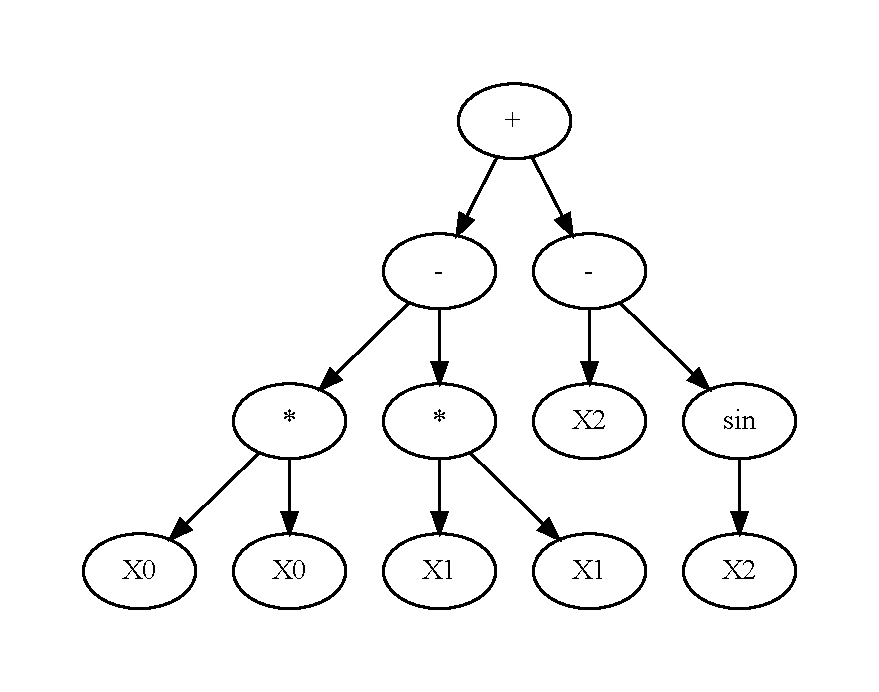
\includegraphics[scale=0.8]{images/graphviz/point_mut_before.dot.pdf}
    \caption{The original expression tree}
    \label{fig:point_muta}
  \end{subfigure}%
  \\
  \begin{subfigure}{\textwidth}
    \centering
    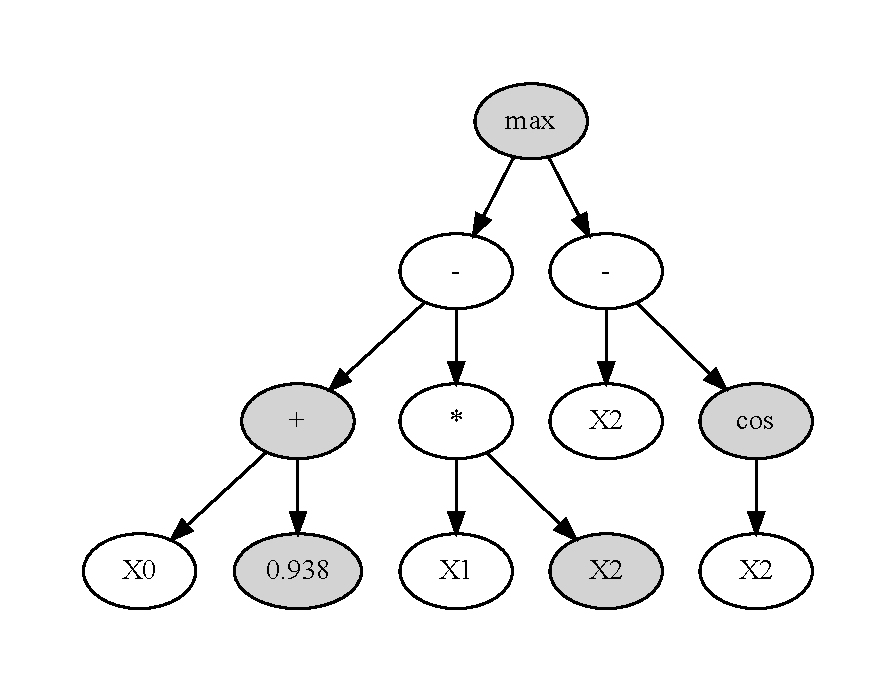
\includegraphics[scale=0.8]{images/graphviz/point_mut_after.dot.pdf}
    \caption{The same expression tree after replacing some nodes(shaded here) with another node of the same arity}
    \label{fig:point_mutb}
  \end{subfigure}
  \caption{Visualizing point mutations}
  
  \label{fig:point_mut}
\end{figure}

\begin{figure}[htp]
  \centering
  \begin{subfigure}{\textwidth}
    \centering
    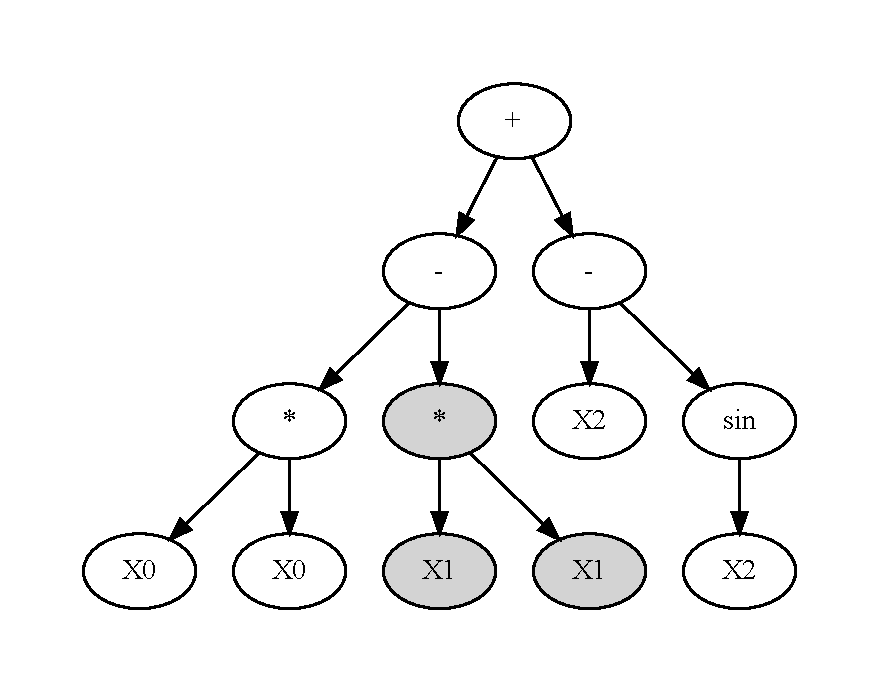
\includegraphics[scale=0.8]{images/graphviz/hoist_mut_before.dot.pdf}
    \caption{The original expression tree. The subtree to be hoisted is highlighted.}
    \label{fig:hoist_muta}
  \end{subfigure}%
  \\
  \begin{subfigure}{\textwidth}
    \centering
    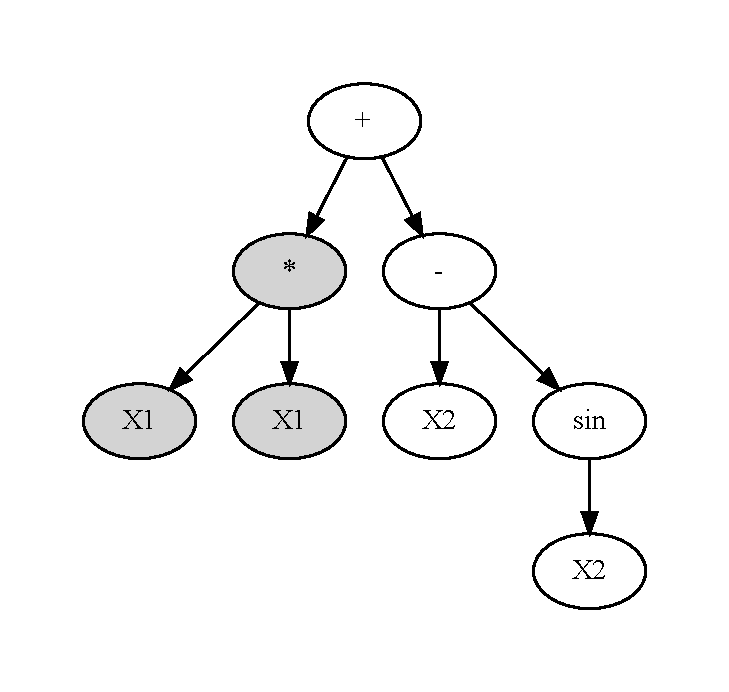
\includegraphics[scale=0.8]{images/graphviz/hoist_mut_after.dot.pdf}
    \caption{The same expression tree after hoisting the subtree}
    \label{fig:hoist_mutb}
  \end{subfigure}
  \caption{Visualizing hoist mutations}
  
  \label{fig:hoist_mut}
\end{figure}

 \begin{table}[htbp]
   \caption{A sample table with a table caption placed
     appropriately. This caption is also very long and is
     single-spaced.  Also notice how the text is aligned.}
   \begin{center}
   \begin{tabular}[c]{|c|r|} \hline
     $x$ & $x^2$ \\ \hline 
     1  &  1   \\
     2  &  4  \\
     3  &  9  \\
     4  &  16  \\
     5  &  25  \\
     6  &  36  \\
     7  &  49  \\
     8  &  64  \\ \hline
   \end{tabular}
   \label{tab:sample}
   \end{center}
 \end{table}
 
 \section{Bibliography with BIB\TeX}
 
 I strongly recommend that you use BIB\TeX\ to automatically generate
 your bibliography.  It makes managing your references much easier.  It
 is an excellent way to organize your references and reuse them.  You
 can use one set of entries for your references and cite them in your
 thesis, papers and reports.  If you haven't used it anytime before
 please invest some time learning how to use it.  
 I've included a simple example BIB\TeX\ file along in this directory
called \verb+refs.bib+.  The \verb+iitmdiss.cls+ class package which
 is used in this thesis and for the synopsis uses the \verb+natbib+
 package to format the references along with a customized bibliography
 style provided as the \verb+iitm.bst+ file in the directory containing
 \verb+thesis.tex+.  Documentation for the \verb+natbib+ package should
 be available in your distribution of \LaTeX.  Basically, to cite the
 author along with the author name and year use \verb+\cite{key}+ where
 \verb+key+ is the citation key for your bibliography entry.  You can
 also use \verb+\citet{key}+ to get the same effect.  To make the
 citation without the author name in the main text but inside the
 parenthesis use \verb+\citep{key}+.  The following paragraph shows how
 citations can be used in text effectively.
 
Here are other references for example.  \citet{viz:mayavi} presents a
Python based visualization system called MayaVi in a conference paper.
\citet{pan:pr:flat-fst} illustrates a journal article with multiple
authors.  Python~\citep{py:python} is a programming language and is
cited here to show how to cite something that is best identified with
a URL. 

The implementation of the algorithm mentioned is to be merged with the \textbf{cuml} data science library(\cite{raschka2020machine})

 
 \section{Other useful \LaTeX\ packages}
 
 The following packages might be useful when writing your thesis.
 
 \begin{itemize}  
 \item It is very useful to include line numbers in your document.
   That way, it is very easy for people to suggest corrections to your
   text.  I recommend the use of the \texttt{lineno} package for this
   purpose.  This is not a standard package but can be obtained on the
   internet.  The directory containing this file should contain a
   lineno directory that includes the package along with documentation
   for it.
 
 \item The \texttt{listings} package should be available with your
   distribution of \LaTeX.  This package is very useful when one needs
   to list source code or pseudo-code.
 
 \item For special figure captions the \texttt{ccaption} package may be
   useful.  This is specially useful if one has a figure that spans
   more than two pages and you need to use the same figure number.
 
 \item The notation page can be entered manually or automatically
   generated using the \texttt{nomencl} package.
 
 \end{itemize}
 
 More details on how to use these specific packages are available along
 with the documentation of the respective packages.
